\section{Implementation, Integration and Test Plan}

Having selected a Client-Server architecture with a Microservices-oriented backend, the implementation, integration, and testing phase requires a structured approach. The development team is split into specialized sub-teams (Backend and Mobile) to ensure focus and avoid task dispersion.

The general development guidelines are presented in the high-level workflow graph below (Figure \ref{fig:implementation_plan}).

\begin{figure}[H]
    \centering
    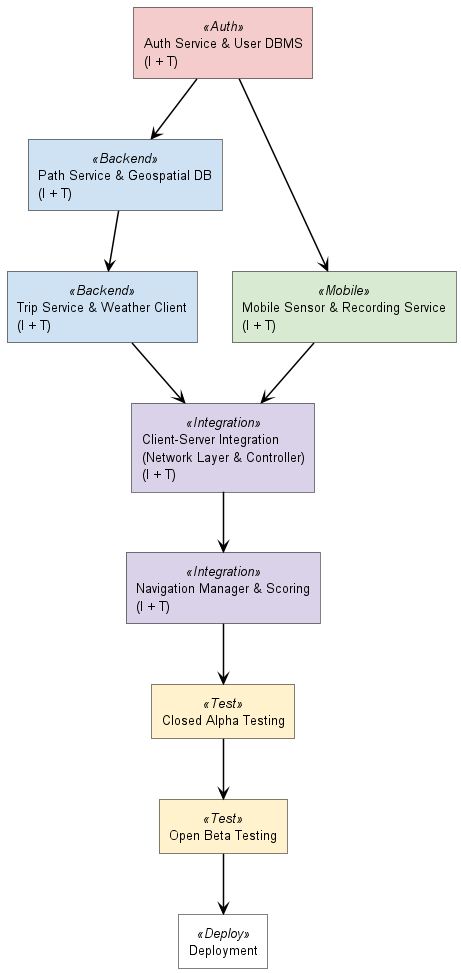
\includegraphics[width=0.7\textwidth]{DD/LaTeXCode/images/ImplementationIntegrationTestPlan/ImplementationIntegrationTestPlan.png}
    \caption{Implementation, Integration and Test Plan Workflow}
    \label{fig:implementation_plan}
\end{figure}

\subsection{Integration Strategy}
The integration follows a \textbf{Bottom-Up Strategy}. Implementation starts from the "leaves" of the hierarchy (independent modules like the Model or Sensor Manager) that do not require other functionalities to work.
These modules require a \textbf{Test Driver} to be developed and tested in isolation. Once a module is validated, it is integrated into the upper layer, eventually replacing the Driver with the actual calling component (e.g., the Controller or UI).

\subsection{Dev-Step 1: Core Infrastructure (Auth \& Data)}
\textbf{Goal:} Establish the persistence layer and user identity management.
\begin{itemize}
    \item \textbf{Activities:} Setup of PostgreSQL. Implementation of \texttt{User Service}, \texttt{Profile Manager}, and the \texttt{Model} repository.
    \item \textbf{Integration:} The \texttt{Auth Service} and \texttt{Profile Manager} are tested via a Driver to verify credential validation and database writes before the API is exposed.
\end{itemize}

\begin{figure}[H]
    \centering
    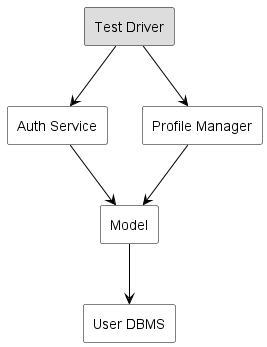
\includegraphics[width=0.5\textwidth]{DD/LaTeXCode/images/ImplementationIntegrationTestPlan/Dev-Step_1_Integration(Auth).png}
    \caption{Dev-Step 1: Auth Integration Tree}
    \label{fig:step1}
\end{figure}

\subsection{Dev-Step 2: Path Management (Backend Stream)}
\textbf{Goal:} Enable the creation and retrieval of \texttt{Path} entities.
\begin{itemize}
    \item \textbf{Activities:} Configuration of PostGIS. Implementation of \texttt{Path Service} and \texttt{Path Searcher}.
    \item \textbf{Integration:} The \texttt{Path Service} is tested via a Driver to verify complex geospatial queries (R7) and visibility logic (R25) against the Database.
\end{itemize}

\begin{figure}[H]
    \centering
    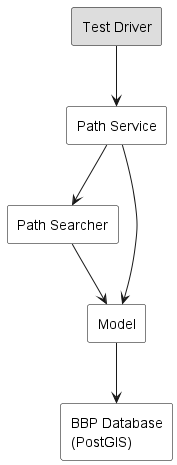
\includegraphics[width=0.5\textwidth]{DD/LaTeXCode/images/ImplementationIntegrationTestPlan/Dev-Step_2_Integration(Path).png}
    \caption{Dev-Step 2: Path Integration Tree}
    \label{fig:step2}
\end{figure}

\subsection{Dev-Step 3: Sensor Abstraction (Mobile Stream)}
\textbf{Goal:} Develop the client-side hardware logic in parallel.
\begin{itemize}
    \item \textbf{Activities:} Implementation of \texttt{Sensor Manager}, \texttt{Recording Service}, and \texttt{Sensor Processor}.
    \item \textbf{Integration:} A Mobile Test Driver simulates UI commands (Start/Stop) to verify that the \texttt{Recording Service} correctly orchestrates the sensors and persists data to \texttt{Local Storage}.
\end{itemize}

\begin{figure}[H]
    \centering
    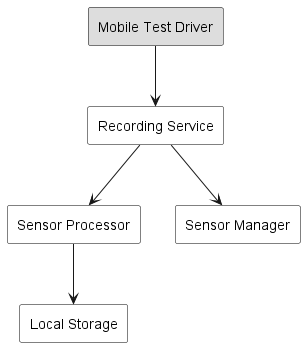
\includegraphics[width=0.5\textwidth]{DD/LaTeXCode/images/ImplementationIntegrationTestPlan/Dev-Step_3_Integration(Mobile Sensors).png}
    \caption{Dev-Step 3: Sensor Logic Integration Tree}
    \label{fig:step3}
\end{figure}

\subsection{Dev-Step 4: Trip Logic \& External Services}
\textbf{Goal:} Connect recorded data to backend persistence and external APIs.
\begin{itemize}
    \item \textbf{Activities:} Implementation of \texttt{Trip Service} and the \texttt{Weather API Client}.
    \item \textbf{Integration:} The \texttt{Trip Service} is tested to ensure it correctly links new Trips to Users and Paths in the \texttt{Model}, and successfully fetches data from the \texttt{Weather Client}.
\end{itemize}

\begin{figure}[H]
    \centering
    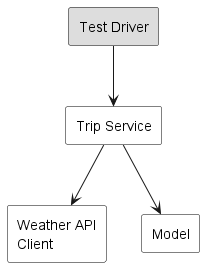
\includegraphics[width=0.5\textwidth]{DD/LaTeXCode/images/ImplementationIntegrationTestPlan/Dev-Step_4_Integration(Trip & Weather).png}
    \caption{Dev-Step 4: Trip Integration Tree}
    \label{fig:step4}
\end{figure}

\subsection{Dev-Step 5: System Integration (The Merge)}
\textbf{Goal:} Remove Drivers and connect the Mobile Client to the Backend.
\begin{itemize}
    \item \textbf{Activities:} Implementation of the \texttt{Controller Layer} and Mobile \texttt{Network Layer}.
    \item \textbf{Integration:} The Test Drivers have been removed. The Mobile \texttt{UI Layer} now communicates through the \texttt{Network Layer} to the \texttt{Controller}, which routes requests to the fully integrated backend services.
\end{itemize}

\begin{figure}[H]
    \centering
    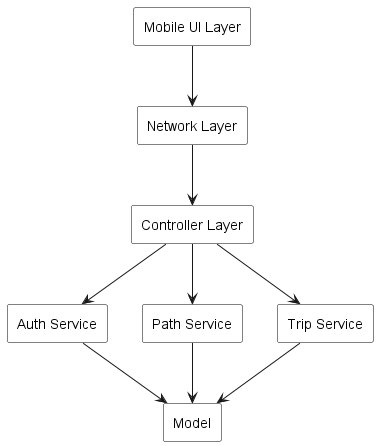
\includegraphics[width=0.7\textwidth]{DD/LaTeXCode/images/ImplementationIntegrationTestPlan/Dev-Step_5(System Integration).png}
    \caption{Dev-Step 5: Full System Integration}
    \label{fig:step5}
\end{figure}

\subsection{Dev-Step 6 \& 7: Advanced Features \& Release}
With the core system integrated, the final steps focus on:
\begin{itemize}
    \item \textbf{Features:} Adding \texttt{Navigation Manager} and \texttt{Scoring Logic} (R9, R10).
    \item \textbf{Closed Alpha:} Distributed to the development team to identify blocking bugs.
    \item \textbf{Open Beta:} Released to a limited user base to stress-test the database under concurrent load.
\end{itemize}